% -*- TeX-master: "ijcai18.tex" -*-

\section{Introduction}\label{sec:intro}

Rule-based modeling languages for molecular biology, such as Kappa \cite{DanosEtAl-CONCUR07} and BioNetGen \cite{bngl}, or organic chemistry, such as M{\o}d \cite{moll}, can be used to write mechanistic models of complex reaction systems. These approaches consider entities that have a structure, and a distinction is made between the transformation of a structure fragment (a pattern), specified by a rule, and the reaction resulting from the application of the rule to a combination of entities contextualizing the fragment. The structure of bio-molecular entities is conveniently represented as a graph and a rule is a graph-rewrite directive with a rate constant that determines its propensity to apply. The stochastic simulation of a rule collection generates a time series of rule applications---henceforth events---that might reach a state of interest in processes like the assembly of a molecular machine, the activation of a transcription factor, or the synthesis of a specific chemical compound. 

% Add a picture of a large story ? - Takes to much space...
% \begin{figure}[!h]
  \vskip -0.1cm
  \begin{center}
    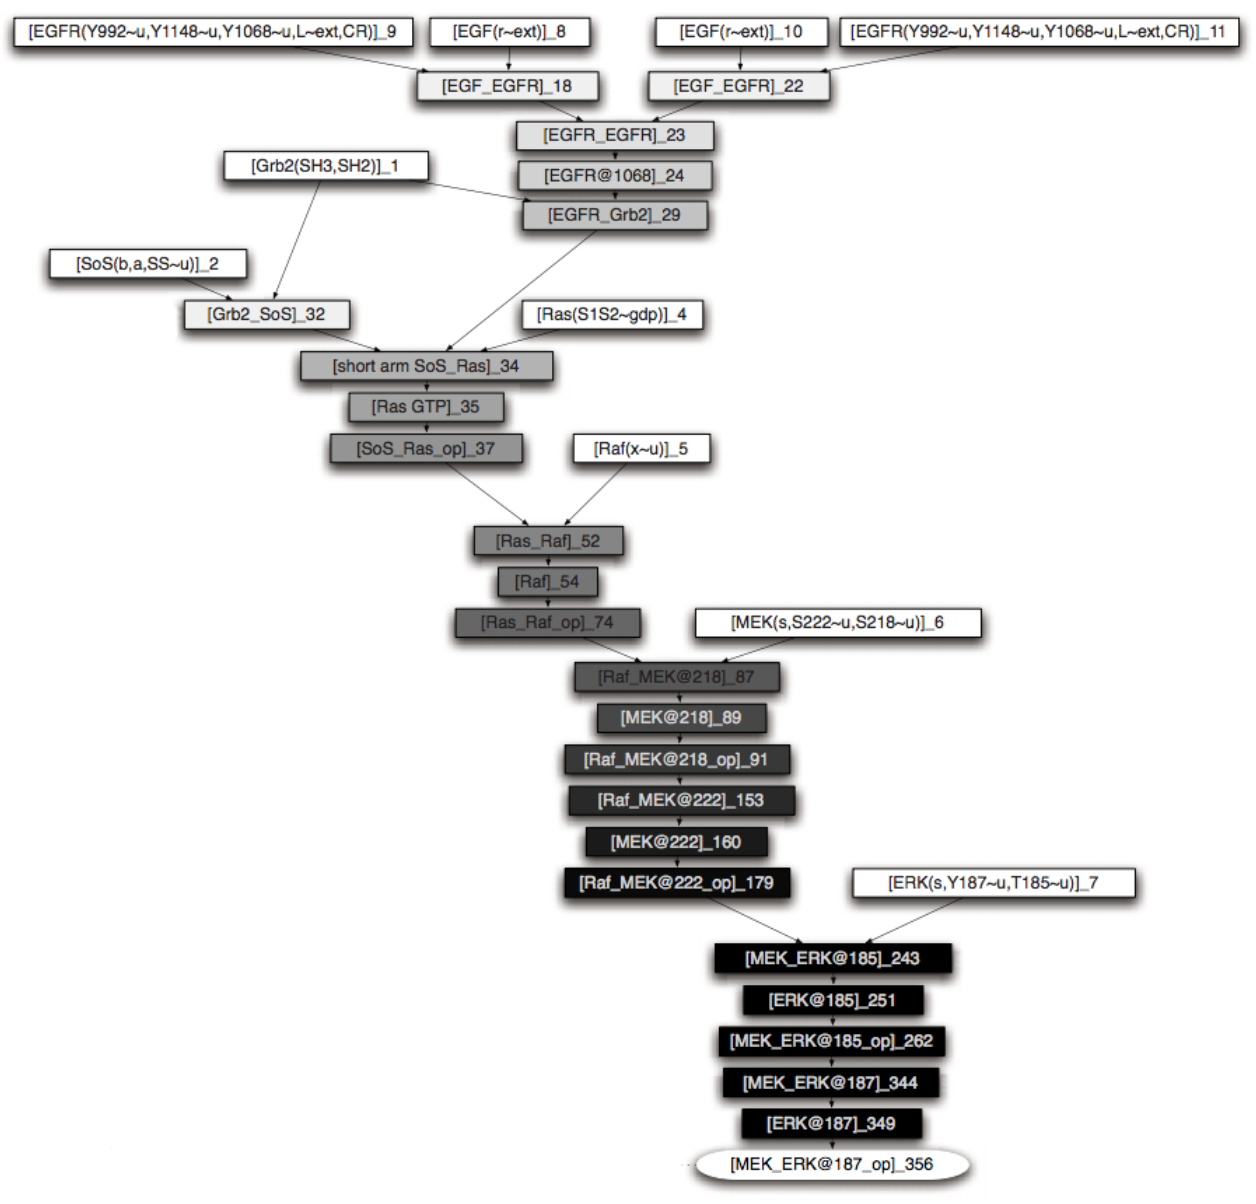
\includegraphics[scale=0.35]{figures/story-egfr.png}
  \end{center}
  \vskip -0.1cm
  \caption{An example of a story describing a part of the EGFR
    signalling pathway, adapted from
    \protect\cite{DanosEtAl-CONCUR07}. Rectangles correspond to
    individual events and solid arrows denote activation between
    them. }
  \label{fig:story-egfr}
\end{figure}


While rule-based models provide compactness, transparency, and the ability of handling combinatorial complexity, the perhaps most significant advantage lies in their suitability for causal analysis. This is because such analysis proceeds at the level of rules and not reactions, thereby avoiding contamination with context that defines a reaction yet is accidental to the application of the underlying rule. Due to the concurrent nature of events it is typically far from obvious how a given series of events attained a particular outcome. Biologists often refer to a causal account or explanation as a ``pathway", but have no formal framing for it.

The approach to causal analysis provided in \cite{DBLP:conf/fsttcs/DanosFFHH12,DanosEtAl-CONCUR07} takes advantage of rule structure to
\begin{inparaenum}[(i)]
\item \label{step:compress} compress a simulation trace into a
  minimal subset of events that are necessary and jointly sufficient
  to replicate the outcome of interest and
\item \label{step:highlight} highlight causal influences between
events, exposing the extent of concurrency.
\end{inparaenum}
Such analysis is usually performed on a large sample of traces to the outcome, thus recovering the salient pathways as those that are statistically favored by the dynamics. This approach, however, suffers from two drawbacks. First, the focus on necessity in step (\ref{step:compress}) neglects events that are kinetically critical (in that they dramatically increase the probability of observing the outcome), yet are not logically necessary for achieving it. Second, step (\ref{step:highlight}) is limited to a narrow notion of causal influence that we may call \emph{activation}. Put simply, an event $a$ is said to activate event $b$, if $a$ modifies an aspect of the state of the world in such a way as to directly enable $b$ to happen. This positively tinted version of influence is blind to the ubiquitous role of \emph{inhibition} in molecular biology.  Indeed, an event $a$ may cause an event $b$ without (transitively) activating it, but instead by preventing another event $c$ that would have prevented $b$. Clearly, uncovering such an explanatory narrative is challenging because it involves events that may \emph{not} occur in a trace ($c$ in this case).

We here propose an approach based on counterfactual reasoning that complements the existing causal analysis of event series generated from rule-based models. In the tradition of Lewis, Pearl and Halpern, we investigate possible causal influences by answering questions of the kind: \textit{Had event $e_1$ not occurred, would event $e_2$ have happened?}
% \cite{lewis1974causation,pearl2009causality,halpern2016actual},
Our contributions are as follows.
\begin{enumerate}
\item We provide a semantics for counterfactual statements in the context of rule-based models, where the standard definition of counterfactuals based on structural equations \cite{pearl2009causality} does not apply.
\item We show how such statements can be evaluated by sampling
\emph{counterfactual traces} that are meant to probabilistically ``hug" a given (factual) trace as much as an external intervention permits them to. To this end, we introduce an algorithm to generate counterfactual traces and provide an efficient implementation for the Kappa language.
\item We show how counterfactual dependencies between events give rise to explanations that include a combination of activating and inhibiting influences that are more in line with biological reasoning.
\end{enumerate}
